\section{Problem 3}

\lstinputlisting{p3.py}
We set out to solve the given ordinary differential equation (ODE) given in
the handout. I have very little to show--I do not have the analytic solution,
and it is clear from \autoref{rk} that the solution is not correct. My attempt
was to decompose the second-order ODE to a first-order, then to use the
Runge-Kutta fourth-order algorithm to solve the ODE. Results are below.
I needed much more help than I sought out, I recognize that. But, it was also
important to try and do the rest of the assignment as well...

\begin{figure}[h!]
    \centering
    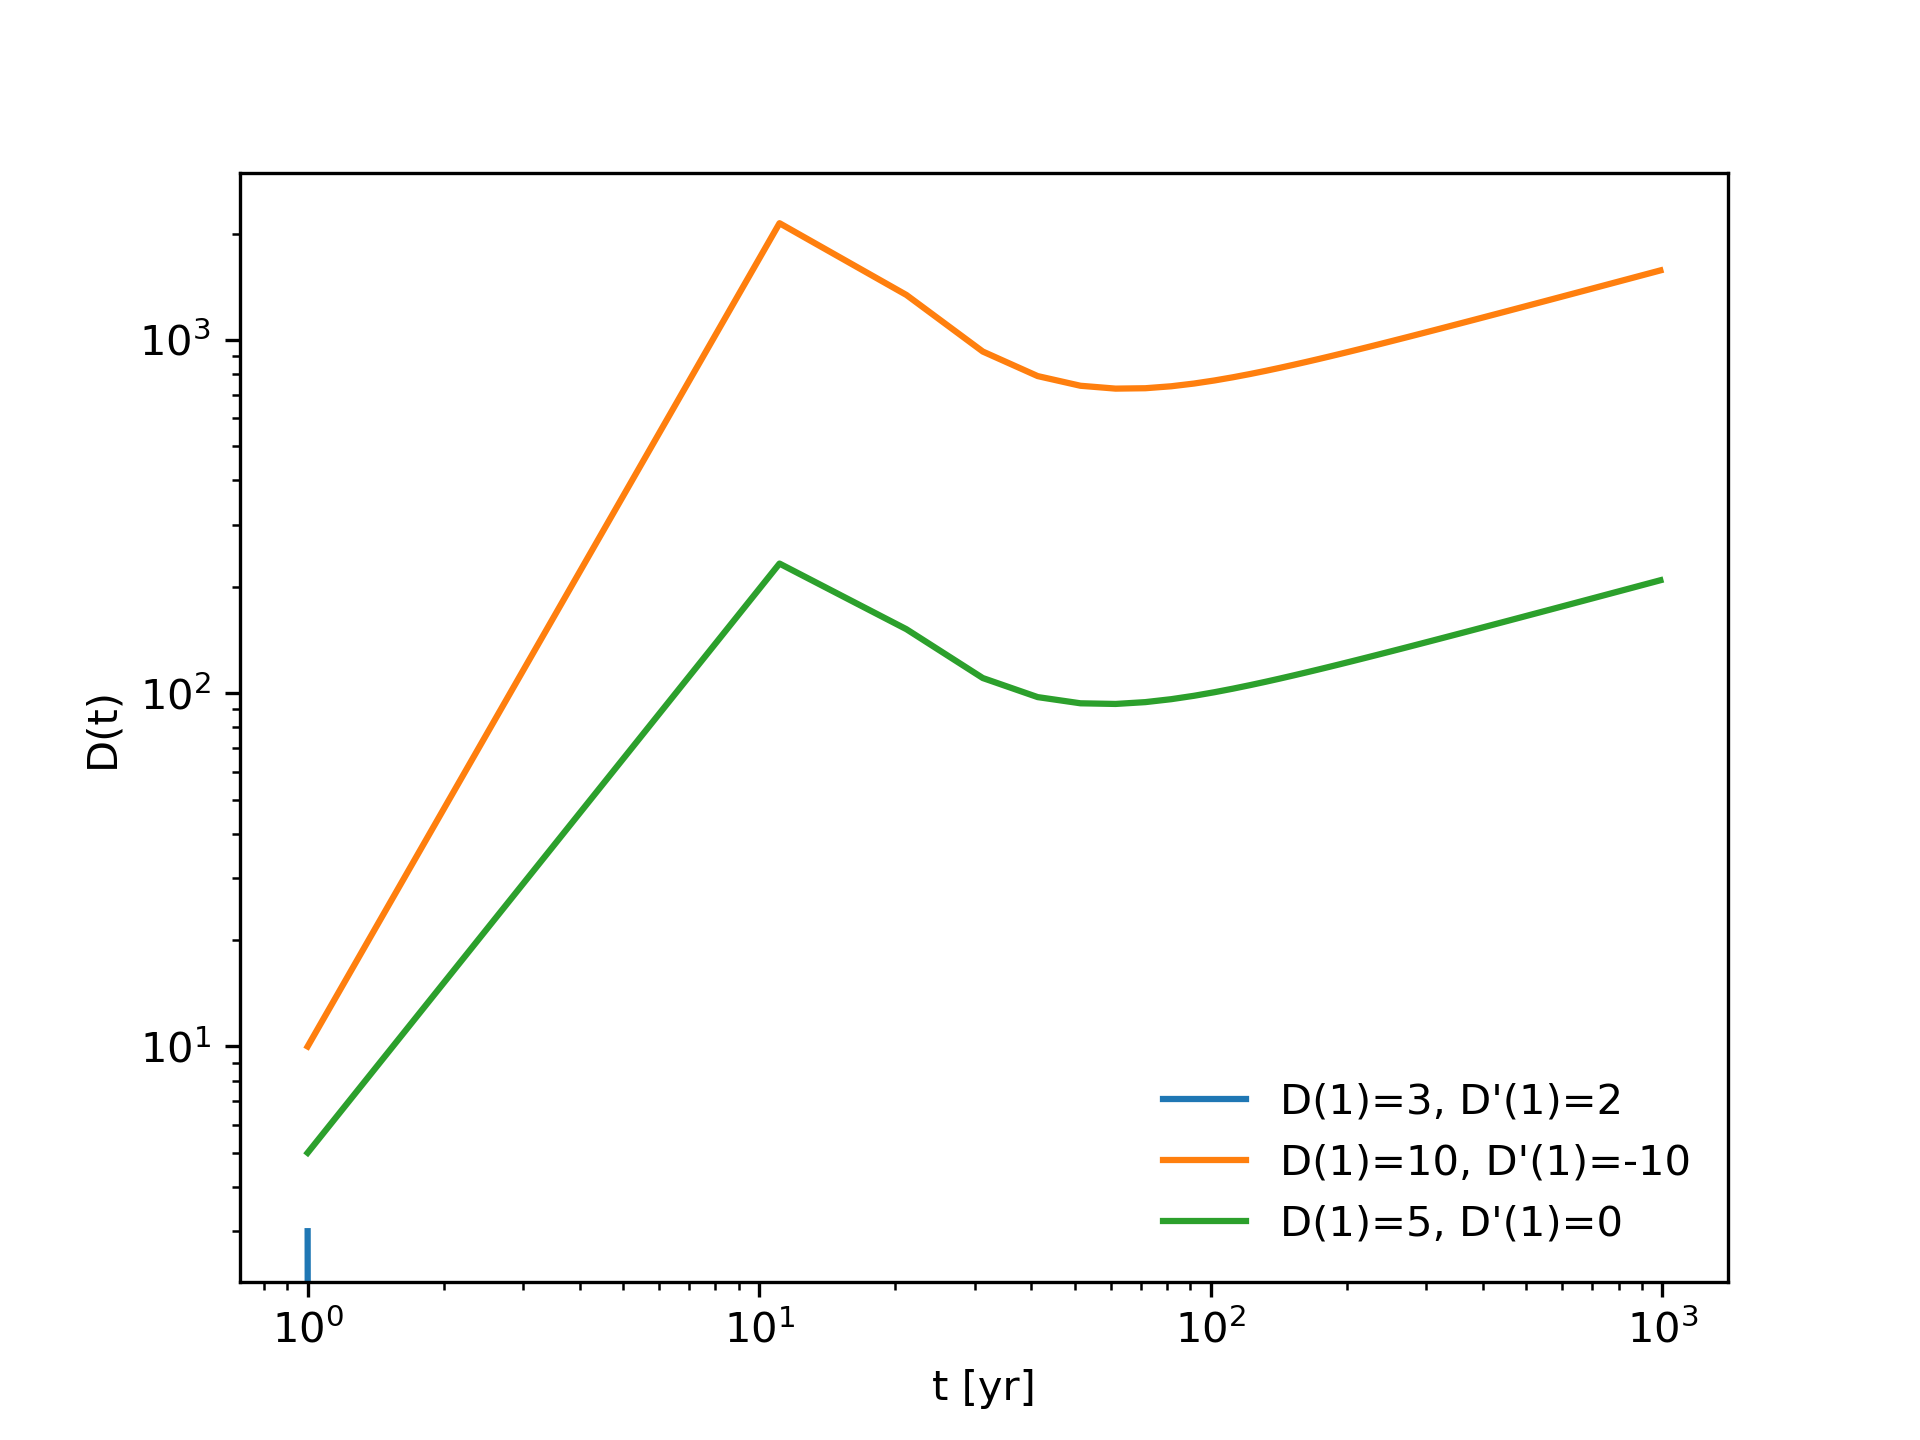
\includegraphics[width=0.9\linewidth]{./plots/rk4.png}
    \caption{Sad plot of the ODE solved.}
    \label{rk}
\end{figure}

